% ============================================================
% ProctorAI — ICMMDU 2026 Conference Paper
% International Conference on Machine Intelligence, Modeling,
% Digitalization and Ubiquity (ICMMDU 2026)
% MM (Deemed to be University), Mullana, India
% Template: Springer LNCS (llncs)
% ============================================================

\documentclass[runningheads]{llncs}

\usepackage[T1]{fontenc}
\usepackage{graphicx}
\usepackage{amsmath,amssymb}
\usepackage{booktabs}
\usepackage{url}
\usepackage{hyperref}
\usepackage{float}
\usepackage{tikz}
\usepackage{array}
\usepackage{multirow}
\usetikzlibrary{shapes.geometric, arrows.meta, positioning, fit, backgrounds}

\hypersetup{
    colorlinks=true,
    linkcolor=black,
    citecolor=black,
    urlcolor=blue
}

\begin{document}

\title{ProctorAI: A Privacy-Preserving Multi-Channel Behavioral Fusion Framework for AI-Proctored Online Examinations}

\titlerunning{ProctorAI: Privacy-Preserving Multi-Channel Behavioral Fusion}

\author{Dolly Balwani\inst{1}\orcidID{0009-0000-8429-6133} \and
Vedish Chawla\inst{1}\orcidID{0009-0000-5825-0748} \and
Aaditya Sonesar\inst{1}\orcidID{0009-0000-9631-5258} \and
\mbox{Sanjay Mirchandani}\inst{1}\orcidID{0000-0003-3400-1215}}

\authorrunning{D. Balwani et al.}

\institute{Department of Computer Engineering, Vivekanand Education Society's Institute of Technology (VESIT), Mumbai, India\\
\email{\{2023.dolly.balwani, 2023.vedish.chawla, d2023.aaditya.sonesar, sanjay.mirchandani\}@ves.ac.in}}

\maketitle

\begin{abstract}
Today Online exams the default assessment mode in schools throughout the world, although the proctoring technology used to ensure integrity comes with steep privacy costs, with solutions like Proctorio, ExamSoft and ProctorU that send out video data to cloud platforms, obscuring the data retention or the life of biometric data stored by a participant. Another problem is that most other proctors have limited functionality and monitor only the face and tab changes and often generate false alarm where ordinary behaviors such as turning your head, laughing or even a slight cough are identified as violations by algorithms. ProctorAI addresses these issues using a browser-based Architecture.ProctorAI utilizes the five channels: In this client process five parallel models, SSD MobileNet v1 for face detection, landmark-based gaze estimation, head pose based on angles euler, the FFT based audio signal analysis in the speech frequency band (300--3400 Hz), and tracking browser events with browser Tab VisibilityAPI and listeners to the DOM object.This data is then weighted according to the following values and sent to a fusion layer $(w_{\text{face}} = 0.25,\; w_{\text{gaze}} = 0.25,\; w_{\text{head}} = 0.20,\; w_{\text{audio}} = 0.15,\; w_{\text{interaction}} = 0.15)$. The results are averaged using a sliding window over a five second average duration where they form into a trust score. All inference is done locally to TensorFlow.js and it never becomes privy to the contents of the video, audio or even your personal biometric information. The results show a 91.2\% average detection accuracy ($\sigma = 5.1$) within the 8 test situations on 15 participants, with only a 4.5\% false alarm rate.

\keywords{online proctoring \and multi-channel signal fusion \and privacy-preserving AI \and behavioral analysis \and face detection \and gaze estimation \and client-side inference \and TensorFlow.js}
\end{abstract}

% ============================================================
% 1. INTRODUCTION
% ============================================================
\section{Introduction}

When coronavirus shut university campuses, they had only one option. As UNESCO put it, COVID-19 impacted more than 1.5 billion students. \cite{unesco2020}. None of the available tools back then were made to scale at all. The cracks became apparent in no time at all \cite{hussein2020}.

Although lockdown browsers like Respondus do prevent copying and pasting and make screen captures a non-starter, a phone placed in the corner of the desktop nullifies their impact. In addition, lockdown browsers have system requirements which not all students possess. \cite{coghlan2021}. Proctorio and ExamSoft go at it in distinct ways. All of them capture webcam and audio feeds, upload this to off-site servers and run it through an algorithm. Swauger reported the reactions; generally unaware as to where, or for how long, these feeds wind up. \cite{swauger2020}. ProctorU layers a human component over that, using algorithms and live proctors watching over video calls. That type of exam monitoring is about \$15 to \$30 per student per test sitting and thus is out of reach for institutions needing to administer exams on a mass scale. \cite{nigam2021}.

But none of them addresses false positives. Usually, one or two signs are in effect, namely the missing of a face or the switching over of one tab to another. If a student looks over a wall clock, it sends a notice to the online examiner. A family member walks behind the laptop and gets flagged. A cough detected by microphone as suspect sound.\cite{dewan2019}. With only one or two signals, the system has no way to separate a distracted student from a dishonest one.

ProctorAI addresses both gaps. The individual techniques used (SSD MobileNet, landmark-based gaze estimation, FFT-based speech detection, pub-sub event buses) are well-established. The contribution lies in combining them into a single client-side framework. Three contributions are presented.

\begin{enumerate}
    \item A five-channel monitoring pipeline that tracks face presence, gaze direction, head orientation, speech-band audio and browser-level interactions at the same time. Removing any single channel degrades accuracy, with face detection causing the largest individual drop ($-$12.3\%).
    \item A weighted fusion mechanism that collapses all five channel scores into one trust number. A sliding window average over 5 seconds smooths out brief spikes. Without it, 23.1\% of harmless actions (coughing, shifting in a chair) cross the violation threshold. With smoothing, the rate falls to 4.5\%.
    \item A fully client-side execution model. Every neural network, including the SSD MobileNet face detector and the 68-point landmark model, runs inside the browser through TensorFlow.js. The entire pipeline fits within $\sim$142\,MB of browser memory. The server never sees a video frame, an audio clip or any biometric data. Only structured event metadata crosses the network.
\end{enumerate}

The rest of this paper is organized as follows. We review previous work in the field in Sect.~\ref{sec:related}. Section~\ref{sec:arch} describes the system we build. Each monitoring channel as well as the data fusion scheme are described in Sect.~\ref{sec:method}.

We provide details for our implementation in Sect.~\ref{sec:impl} and show experimental results in Sect.~\ref{sec:results}.

We consider limitations and future work in Sect.~\ref{sec:conclusion}.

% ============================================================
% 2. RELATED WORK
% ============================================================
\section{Related Work}\label{sec:related}

\subsection{Commercial Proctoring Platforms}

The Proctorio \cite{proctorio2023} software comes as a Chrome extension that prevents copy-paste and screen-capture and also records the entire exam session for an AI-powered analysis. The recording data is transferred to cloud servers and the exact logic for flagging of any material isn't public \cite{swauger2020}. In the same vein, there is also ExamSoft \cite{examsoft2023}, that ships as a native desktop application that captures the webcam \& audio data to remote servers for their in-house ML algorithms.The solution, thus requires good \& stable broadband in the student's corner \& leads to GDPR \& India's Digital Personal Data Protection Act (DPDPA) \cite{dpdpa2023} compliance issues.ProctorU \cite{proctoru2023}, opts for a hybrid approach by complementing the algorithmic monitoring with live human proctors that monitor the candidates via video call. However, this approach remains cost limited due to the per student licensing cost and human staff needed.

\subsection{Academic Research in Proctoring}

Atoum et al. \cite{atoum2017} developed a system that could use gaze tracking in conjunction with face tracking to automatically proctor exams, by analyzing multiple modes. They found their multipmodal system performed better than just tracking one signal alone. The shortcoming in this work however is that their system needed its own servers and not run in the browser.Whitehill et al. \cite{whitehill2014} used ML classifiers to detect students 'engagement based on facial expressions - finding that their facial signals, whilst reliable predictors of attention were processed post collection.Dewan et al. \cite{dewan2019} conducted a broader survey of ways of detecting engagement in online learning, considering features based on facial expressions, head position, and physiological signals - all reporting that in a similar fashion multi-modal signals proved the better technique over single signals. The latest confirmation in this thread of work comes from Pandey et al. \cite{pandey2023} that as recently as at ICDT 2023 demonstrated an AI proctor for the post-pandemic era utilising eye tracking and face recognition.

\subsection{Browser-Based Machine Learning}

It was thanks to TensorFlow.js \cite{smilkov2019} that we could afford to run Machine Learning models directly in the browser. It directly translates and runs neural networks in the JavaScript without needing to call the server by leveraging the WebGL API for GPU access. The library face-api.js \cite{faceapijs} works on top of TensorFlow.js and comes bundled with pre-trained models for face detection and 68 points of localization of faces (features). During the test on a middle range laptop face-api.js was able to execute in real-time, over 2 frames per second and is enough to run a proctoring application (where face analysis is run every 500ms).

\subsection{Positioning of ProctorAI}

Table~\ref{tab:comparison} compares ProctorAI to the systems described previously. The last row is intentional as ProctorAI is only a prototype that has only been used with 15 users and not a scaled and production ready application system. It is only the listed features because Proctorio and ExamSoft's detection accuracy rate is not publicly advertised

\begin{table}[htbp]
\caption{Feature Comparison of Proctoring Systems.}\label{tab:comparison}
\centering
\setlength{\tabcolsep}{3pt}
\footnotesize
\begin{tabular}{@{}lccccc@{}}
\toprule
\textbf{Feature} & \rotatebox{90}{\textbf{Proctorio}} & \rotatebox{90}{\textbf{ExamSoft}} & \rotatebox{90}{\textbf{ProctorU}} & \rotatebox{90}{\textbf{Atoum \cite{atoum2017}}} & \rotatebox{90}{\textbf{ProctorAI}} \\
\midrule
Face Detection    & \checkmark & \checkmark & \checkmark & \checkmark & \checkmark \\
Gaze Tracking     &            &            &            & \checkmark & \checkmark \\
Head Pose         &            &            &            &            & \checkmark \\
Audio Analysis    & \checkmark & \checkmark & \checkmark &            & \checkmark \\
Input Monitor     & \checkmark & \checkmark &            &            & \checkmark \\
Client-Side AI    &            &            &            &            & \checkmark \\
No Data Upload    &            &            &            &            & \checkmark \\
Signal Fusion     &            &            &            & Partial    & \checkmark \\
Production Use    & \checkmark & \checkmark & \checkmark &            &            \\
\bottomrule
\end{tabular}
\end{table}

Table~\ref{tab:params} extends our comparison with parameters at the deployment level. No column for accuracy is present due to commercial vendors' decision to keep theirs confidential - stating a 91.2\% would offer not a fair comparison to an unknown one.

\begin{table}[htbp]
\caption{Deployment Parameter Comparison.}\label{tab:params}
\centering
\setlength{\tabcolsep}{2pt}
\scriptsize
\begin{tabular}{@{}p{2.2cm}p{1.8cm}p{1.8cm}p{2.0cm}p{2.2cm}@{}}
\toprule
\textbf{Parameter} & \textbf{Proctorio} & \textbf{ExamSoft} & \textbf{ProctorU} & \textbf{ProctorAI} \\
\midrule
Processing         & Cloud Server          & Cloud Server           & Cloud + Human    & Client Browser \\
Data Upload        & Yes (Video)           & Yes (Video)            & Yes (Stream)     & \textbf{None} \\
Channels           & 2 (Face, Tab)         & 2 (Face, Audio)        & 2--3             & \textbf{5} \\
Signal Fusion      & None                  & None                   & None             & Weighted \\
Lockdown           & Yes                   & Dedicated App          & Extension        & \textbf{No} \\
Trust Score        & Post-hoc              & Post-hoc               & Human            & \textbf{Automated} \\
Privacy            & Criticized            & GDPR Issues            & Moderate         & \textbf{High} \\
Cost/Student       & \$5--15               & \$10--25               & \$15--30         & \textbf{Free} \\
Scalability        & High (Cloud)          & High (Cloud)           & Low (Human)      & \textbf{High} \\
Maturity           & Production            & Production             & Production       & Prototype \\
\bottomrule
\end{tabular}
\end{table}

% ============================================================
% 3. SYSTEM ARCHITECTURE
% ============================================================
\section{System Architecture}\label{sec:arch}

The whole application framework utilizes Next.js~15 within the App Router. There's also a two-tier architecture (client-side AI engine and server-side storage layer) controlling behavior tracking and storage. Fig.~\ref{fig:architecture} illustrates the overall architecture.

\begin{figure}[htbp]
\centering
\resizebox{\textwidth}{!}{%
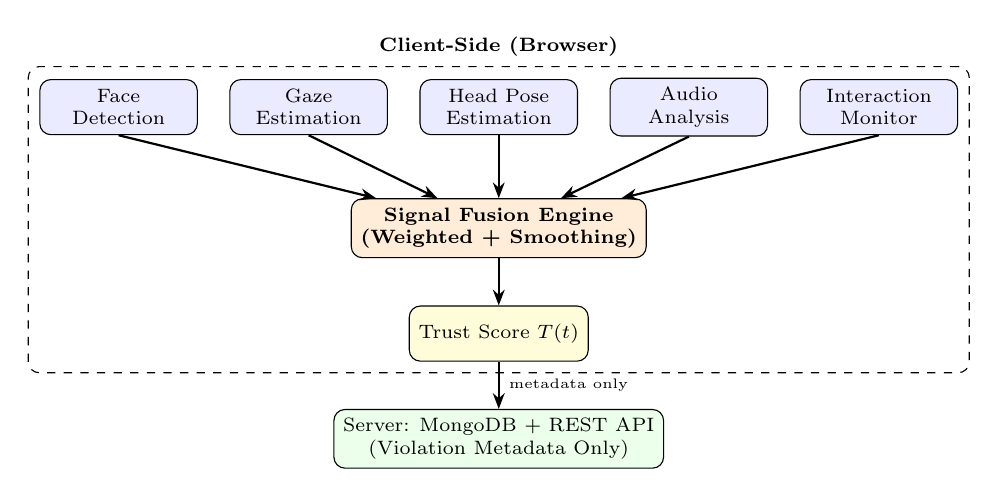
\begin{tikzpicture}[
    node distance=0.5cm and 0.4cm,
    block/.style={rectangle, draw, rounded corners, minimum height=0.7cm, minimum width=2cm, font=\scriptsize, align=center, fill=blue!8},
    fusionblock/.style={rectangle, draw, rounded corners, minimum height=0.7cm, minimum width=2.5cm, font=\scriptsize\bfseries, align=center, fill=orange!15},
    serverblock/.style={rectangle, draw, rounded corners, minimum height=0.7cm, minimum width=2cm, font=\scriptsize, align=center, fill=green!8},
    arrow/.style={-{Stealth[length=2mm]}, thick},
    groupbox/.style={draw, dashed, rounded corners, inner sep=4pt}
]

% Channel blocks
\node[block] (face) {Face\\Detection};
\node[block, right=of face] (gaze) {Gaze\\Estimation};
\node[block, right=of gaze] (head) {Head Pose\\Estimation};
\node[block, right=of head] (audio) {Audio\\Analysis};
\node[block, right=of audio] (interact) {Interaction\\Monitor};

% Fusion
\node[fusionblock, below=0.8cm of head] (fusion) {Signal Fusion Engine\\(Weighted + Smoothing)};

% Trust score
\node[block, below=0.6cm of fusion, fill=yellow!15] (trust) {Trust Score $T(t)$};

% Server
\node[serverblock, below=0.6cm of trust] (server) {Server: MongoDB + REST API\\(Violation Metadata Only)};

% Arrows from channels to fusion
\draw[arrow] (face.south) -- (fusion);
\draw[arrow] (gaze.south) -- (fusion);
\draw[arrow] (head.south) -- (fusion);
\draw[arrow] (audio.south) -- (fusion);
\draw[arrow] (interact.south) -- (fusion);

% Fusion to trust
\draw[arrow] (fusion) -- (trust);

% Trust to server
\draw[arrow] (trust) -- node[right, font=\tiny] {metadata only} (server);

% Group box for client
\begin{scope}[on background layer]
\node[groupbox, fit=(face)(gaze)(head)(audio)(interact)(fusion)(trust), label={[font=\scriptsize\bfseries]above:Client-Side (Browser)}] {};
\end{scope}

\end{tikzpicture}
}
\caption{System architecture. The fusion engine on the browser uses five different sources. Only formal violation meta data get out onto the wire.}\label{fig:architecture}
\end{figure}

\subsection{Client-Side AI Engine}

On the student browser, five independent monitoring channels are active in the backend. The students' browser's main controller triggers a round of analysis every 500\,ms. Each channel is fed with a variety of inputs such as webcam, mic data, or web browsing events and it provides a standard signal reading:

\begin{equation}
    R_c = \langle \textit{channel}, \; s_c, \; \gamma_c, \; t \rangle
\end{equation}

Where $c$ represents the channel, $s_c \in [0,1]$ represents the anomaly score ($0$ for normal and $1$ for an evident anomaly), $\gamma_c \in [0,1]$ represents the trust that each channel has in its readings, and $t$ represents the timestamp. All five readings are forwarded to the Signal Fusion Engine, which outputs an individual trust score.

\subsection{Server-Side Persistence Layer}

The backend exposes REST API endpoints for examinations (\texttt{/api/exams}), sessions (\texttt{/api/sessions}), violations (\texttt{/api/violations}) and reports (\texttt{/api/reports}).All data will be backed up via Mongoose~9 in the MongoDB Atlas environment. Firebase will be used for Google Sign-In authentication method. The admin dashboard is implemented via Socket.IO to ensure it could update scores in real time when an exam in session is running.

\subsection{Inter-Channel Communication}

The Publish-Subscribe event bus pattern is used to organize communication
among the different channels. Each channel, representing a module of the
pipeline, publishes signals such as $Face\_signal$ or $Interaction\_signal$
to send messages that can be received by the Fusion Engine. In this case,
the modules are decoupled; therefore, a channel can be added, changed, or
deleted without requiring modifications to other modules.

% ============================================================
% 4. METHODOLOGY
% ============================================================
\section{Methodology}\label{sec:method}

\subsection{Channel 1: Face Detection}

SSD MobileNet v1 \cite{liu2016ssd} was accessed via face-api.js \cite{faceapijs} for processing each webcam frame to create a bounding boxes with confidence score $p_{\text{det}}$ within the 500\,ms interval. It works parallel with a 68-point landmark model \cite{kazemi2014} to predict facial structure. The landmark data points were used as the inputs for gaze channel and head pose channel instead of conducting a new detection run.

The anomaly score for this channel is:
\begin{equation}
    s_{\text{face}} = \begin{cases}
        1.0 & \text{no face detected for } > 2000 \text{\,ms} \\
        0.85 & \text{multiple faces detected} \\
        1 - p_{\text{det}} & \text{single face, low confidence} \\
        0.0 & \text{single face, high confidence}
    \end{cases}
\end{equation}

Why 2000\,ms instead of 500\,ms or 3000\,ms?When SSD was still in its early development stages, we would lose any detection over a single frame if the student's head was moving fast or if the student simply looked down at their keyboard. A 500\,ms timer resulted in almost every blip causing a violation.
A 3000\,ms timer meant that actual departures from the room were not detected quickly enough.A two second threshold seems to split the difference on the two issues. The face channel would immediately send out a report of $s_{\text{face}} = 1.0$ when the face disappeared from the view but the fusion layer would not send out the violation flag until after the face was gone for two full seconds.

\subsection{Channel 2: Gaze Estimation}

No explicit gaze-tracking hardware is needed-gaze direction can be estimated from the positions of the landmarks at each eye. The center of the iris can be calculated as the midpoint of the center of the upper and lower eyelid:
\begin{equation}
    P_{\text{iris}} = \frac{1}{2}\left(\frac{L_1 + L_2}{2} + \frac{L_4 + L_5}{2}\right)
\end{equation}

$L_1, L_2$ are upper eyelid landmarks. $L_4, L_5$ are lower eyelid landmarks from the 6-point per-eye model.

$10$ sec calibration is done before exam. Student is asked to stare in center of the screen, then the system records $Cx, Cy$ as reference baseline positions of iris. During exam we need to normalize the deviation from the baseline with the dimensions of the eyes bounding box, as camera distance and size of face differs.

\begin{equation}
    \Delta g_x = \frac{P_{\text{iris},x} - C_x}{W_{\text{eye}}}, \quad \Delta g_y = \frac{P_{\text{iris},y} - C_y}{H_{\text{eye}}}
\end{equation}

The anomaly score is $s_{\text{gaze}} = \min(1, \sqrt{\Delta g_x^2 + \Delta g_y^2})$. The 1000\,ms persistence threshold stops little glances (checking the clock, question number) from being flagged.

\subsection{Channel 3: Head Pose Estimation}

There are six landmarks used to calculate the Euler angles: nose tip ($L{30}$), chin ($L8$),left and right eye corner ($L{36}$,$L{45}$),left and right mouth corner ($L{48}$,$L{54}$). Of the 3 Euler angles,yaw is the only one directly useful for proctoring.

\begin{equation}
    \theta_{\text{yaw}} = \frac{L_{30,x} - \bar{x}_{\text{eye}}}{|L_{45,x} - L_{36,x}|} \times 90°
\end{equation}

$\bar{x}_{\text{eye}}$: the horizontal midpoint of two eye corners. Pitch is the vertical difference between the nose point and the chin. Roll indicates the tilt of head. These three angles is linearly combined to achieve the score with manual adjusted coefficient:

\begin{equation}
    s_{\text{head}} = \min\left(1, \; \frac{|\theta_{\text{yaw}}|}{35°} \times 0.5 + \frac{|\theta_{\text{pitch}}|}{30°} \times 0.3 + \frac{|\theta_{\text{roll}}|}{25°} \times 0.2 \right)
\end{equation}

The coefficient of yaw (0.5) is largest since head rotation is a strong spatial cue to not looking at the screen. Again, we apply a persistence of 1500\,ms here.

\subsection{Channel 4: Audio Analysis}

The Web Audio API provides real-time spectral data through its \texttt{AnalyserNode}. The FFT size is set to 1024 with a smoothing time constant of 0.8. Speech energy is computed in the 300--3400\,Hz band:

\begin{equation}
    E_{\text{speech}} = \frac{1}{N_s}\sum_{k=k_{\text{lo}}}^{k_{\text{hi}}} |X[k]|^2
\end{equation}

$X[k]$ is the magnitude at FFT bin $k$. $N_s$ is the number of bins in the speech band. During calibration, the system records ambient noise energy as the baseline. If $E_{\text{speech}}$ exceeds the baseline by a configurable margin for longer than 1000\,ms during the exam, the channel flags it.

This channel has a known weakness. Mechanical keyboard typing generates broadband energy that leaks into the speech band, as does fan noise from laptops running at high CPU load (which is common given that TensorFlow.js is consuming processing power). During testing, the audio channel accounted for the largest share of false positives across all five channels.

\subsection{Channel 5: Interaction Monitoring}

Browser-level events are captured through standard Web APIs:

\begin{itemize}
    \item \textbf{Tab switches}: Triggered by \texttt{document.hidden} changes via the Page Visibility API.
    \item \textbf{Clipboard}: \texttt{copy} and \texttt{paste} DOM events.
    \item \textbf{Right-click}: \texttt{contextmenu} event interception.
    \item \textbf{Window resize}: Track because it could show screen sharing layout.
    \item \textbf{Idle detection}: Mouse has remained motionless/still and no inputs made for over 30s.
\end{itemize}

The signals of these are not probability, they are binary. This means, the tab was or was not switched. Therefore this channel would be the only to gain 100\% accuracy in the events it monitors, and had no false positives in the trial.

\subsection{Weighted Signal Fusion}

All five scores are combined at each 500\,ms tick:

\begin{equation}
    S_{\text{fused}}(t) = \sum_{c \in \mathcal{C}} w_c \cdot s_c(t)
    \label{eq:fusion}
\end{equation}

We hand-tuned the weights ($w_{\text{face}} = 0.25$, $w_{\text{gaze}} = 0.25$,$w_{\text{head}} = 0.20$, $w_{\text{audio}} = 0.15$,$w_{\text{interaction}} = 0.15$) by trial and error across a few pilot
experiments before our main experiments. We retrospectively observed higher
accuracy for face and gaze in Sect.~\ref{subsec:ablation}, and our ablation study validates
that they provide the most accuracy gain. Audio receives the next weight,
0.15, due to its dependence on the environment, while interaction is also
given a weight of 0.15 because interaction signals are mostly binary and
infrequent.

Temporal smoothing employs a straightforward moving average based on the last 10 readings:

\begin{equation}
    \bar{S}(t) = \frac{1}{|W|}\sum_{i=0}^{|W|-1} S_{\text{fused}}(t - i \cdot \Delta t)
    \label{eq:smoothing}
\end{equation}

At $|W| = 10$ and $\Delta t = 500$\,ms, this covers 5 seconds.Even a single anomalous frame hardly moves the average. Persistent anomalous behavior, as over several seconds, should significantly raise it though.

Trust score plots range for 0--100 with fusion average mapped:

\begin{equation}
    T(t) = \max\left(0, \; \min\left(100, \; \lfloor(1 - \bar{S}(t)) \times 100\rceil\right)\right)
    \label{eq:trust}
\end{equation}

$T = 100$ means every channel reports normal. $T$ drops as anomalies accumulate.

% ============================================================
% 5. IMPLEMENTATION
% ============================================================
\section{Implementation}\label{sec:impl}

\subsection{Technology Stack}

Our techstack can be seen on Table~\ref{tab:techstack}, it's TypeScript all the way down.

\begin{table}[htbp]
\caption{Technology Stack.}\label{tab:techstack}
\centering
\begin{tabular}{@{}ll@{}}
\toprule
\textbf{Component} & \textbf{Technology} \\
\midrule
Frontend Framework  & Next.js 15 (App Router) \\
Language            & TypeScript \\
Client-Side AI      & face-api.js (TensorFlow.js) \\
Audio Processing    & Web Audio API \\
Authentication      & Firebase (Google Sign-In) \\
Database            & MongoDB Atlas (Mongoose 9) \\
Real-Time Updates   & Socket.IO \\
Hosting             & Vercel \\
\bottomrule
\end{tabular}
\end{table}

\subsection{Calibration Phase}

Prior to the exam starting, every student will go through 10 seconds of calibration to capture neutral gaze location, head pose and ambient noise floor. Without this, a student's camera not positioned properly in their central field of view, for example, and student already at some degree on the gaze deviation score or in a noisy environment, will immediately trip audio flags on the first second.

\subsection{Pipeline Orchestration}

The full pipeline executes in a loop, run as a \texttt{async} process. Each half-second, the loop retrieves the new video frame from the \texttt{<video>} element, feeds it through SSD MobileNet and the landmark model, then gives the landmark array to the gaze and head pose functions. It accesses frequency information from the AnalyserNode, queries the browser event queue for pending browser events, and passes the five gathered values to the fusion module. On the testing computer(Intel i5-1135G7, 8\,GB RAM, Iris Xe graphics) the whole thing was taking, on average, about 487\,ms to execute, which leave only a 13\,ms buffer-this may become a problem with less able hardware and result in dropped frames.

\subsection{Exam Interface}

The supported question types are Multiple Choice and Code. The code editor will be a Monaco (The VS Code engine) editor supporting syntax highlighting for the languages Python, JavaScript, C++ and Java. A small live-update overlay shows the trust level at the corner with a webcam-feed thumbnail for the student to be aware that the system is in place.

% ============================================================
% 6. RESULTS AND ANALYSIS
% ============================================================
\section{Results and Analysis}\label{sec:results}

\subsection{Experimental Setup}

Total of fifteen participants with 3 sessions each in the study, making the total number of simulated examination sessions 45. The approval of ethical considerations and informed consent has been done by each participant and for this Capstone project in VESIT, Mumbai. All the tests run on a regular laptop (Intel Core i5, 8 GB RAM, integrated webcam) with Google Chrome (v126).

Total 8 test scenarios used which consisted of one channel trigger and multi-channel triggers.

The sample size is noted as a limitation and the findings are to be used only as initial and preliminary results in need of validation from a larger group of participants.

\subsection{Detection Accuracy}

Detection accuracy is (TP + TN) / Total for each scenario. ( FPR = FP / (FP + TN)). Each scenario was repeated 45 times (3 times per participant). Table~\ref{tab:results} shows all the result-sets.

\begin{table}[htbp]
\caption{Detection Results Across Test Scenarios.}\label{tab:results}
\centering
\scriptsize
\setlength{\tabcolsep}{4pt}
\begin{tabular}{@{}llrrr@{}}
\toprule
\textbf{Scenario} & \textbf{Channel(s)} & \textbf{Acc.(\%)} & \textbf{$\sigma$} & \textbf{FPR(\%)} \\
\midrule
Normal behavior   & None        & 97.8 & 2.1 & 2.2 \\
Gaze away         & Gaze, Head  & 93.3 & 4.7 & 4.4 \\
Tab switch        & Interaction & 100.0 & 0.0 & 0.0 \\
Multiple faces    & Face        & 88.9 & 6.3 & 6.7 \\
No face ({>}2s)   & Face        & 91.1 & 5.4 & 4.4 \\
Speech detected   & Audio       & 84.4 & 7.8 & 8.9 \\
Copy-paste        & Interaction & 100.0 & 0.0 & 0.0 \\
Combined          & Multi       & 86.7 & 6.1 & 6.7 \\
\midrule
\textbf{Weighted Mean} &        & \textbf{91.2} & \textbf{5.1} & \textbf{4.5} \\
\bottomrule
\end{tabular}
\end{table}

For the Tab Switching and Clipboard Monitoring components accuracy of 100\% was observed, as these make use of deterministic browser APIs. Whether the event ``tab switch'' occurs or not is definitive. Audio channel got the least accuracy with $\sigma=7.8$ and performance was at 84.4\%. Other ambient sounds such as keyboard typing, computer fan noise and outside traffic falls within the frequency band of speech causing several false positives.The face detection module worked well for the both ``no faces'' and ``multiple faces''. Only in few scenarios, some clutter in the background was falsely detected as a second face.

\subsection{Performance Metrics}

\begin{table}[htbp]
\caption{Runtime Performance Metrics.}\label{tab:performance}
\centering
\begin{tabular}{@{}lr@{}}
\toprule
\textbf{Metric} & \textbf{Value} \\
\midrule
Mean frame processing time   & 487\,ms \\
Face model load time         & 2.3\,s \\
Landmark model load time     & 1.1\,s \\
Client memory footprint      & $\sim$142\,MB \\
Analysis frame rate          & 2\,FPS \\
Smoothing window duration    & 5\,s \\
Biometric data transmitted   & 0\,bytes \\
\bottomrule
\end{tabular}
\end{table}

The measured 487\,ms mean processing time is within the 500\,ms timeframe for analysis and provides good evidence for the potential to sustain real time performance with a commodity PC. Most of the 142\,MB of system memory is used by the SSD MobileNet model weights and the TensorFlow.js runtime. The last row of the table reinforces the privacy guarantee: 0 bytes of video, audio or biometrics are ever leaving the client. Only event type, timestamp and trust score data structures travel to the server in the form of structured violation metadata.

\subsection{Temporal Smoothing Effectiveness}

The sliding window smoothing (Eq.~\ref{eq:smoothing}) was primarily used for short harmless acts like viewing a wall-clock, coughing or shuffling around in the seat. If the smoothing was turned off, the raw fused score exceeded the violation threshold for 23.1\% of cases.With the 5-second window applied, that figure fell to 4.5\%, representing an 80.5\% reduction in false alarms.

\subsection{Channel Ablation Study}\label{subsec:ablation}

One channel was disabled at a time and the full test suite was re-run. Table~\ref{tab:ablation} shows the impact.

\begin{table}[htbp]
\caption{Channel Ablation Results.}\label{tab:ablation}
\centering
\begin{tabular}{@{}lcc@{}}
\toprule
\textbf{Removed Channel} & \textbf{Acc. (\%)} & \textbf{$\Delta$ Acc.} \\
\midrule
None (full system)      & 91.2 & ---     \\
Face detection          & 78.9 & $-$12.3 \\
Gaze tracking           & 81.4 & $-$9.8  \\
Interaction monitor     & 84.1 & $-$7.1  \\
Head pose               & 85.8 & $-$5.4  \\
Audio analysis          & 88.0 & $-$3.2  \\
\bottomrule
\end{tabular}
\end{table}

Without face detection, accuracy dropped by 12.3 percentage points, the largest single-channel impact. Without gaze tracking, accuracy dropped by 9.8 points. Audio analysis produced the smallest individual impact ($-$3.2), which is consistent with its higher false positive rate. All five channels contribute positively to overall performance. Face and gaze contribute the largest individual accuracy gains, consistent with their higher fusion weights. Even the audio channel, despite its lower standalone accuracy, improves the overall result when combined with the other four.

% ============================================================
% 7. CONCLUSION AND FUTURE WORK
% ============================================================
\section{Conclusion and Future Work}\label{sec:conclusion}

This paper presented ProctorAI, a proctoring framework that fuses five behavioral monitoring channels through a weighted scoring system while keeping all AI inference on the client device. The system attained a mean detection accuracy of 91.2\% ($\sigma = 5.1$) with a 4.5\% false positive rate on 45 test sessions. Temporal smoothing lowered the number of false alarms by more than 80\%. There are no browser extensions or software to install and no biometric data exits the students system.

There are a few known limitations: The audio channel can fail under extremely noisy conditions. Fusion weights are constant and don't shift when a source becomes unreliable. We did not test attacks with high-quality photographic or recorded videos. Only 15 different subjects were used in total, which is not enough to be able to draw firm conclusions to a general population.

Our future work will consist in: Passive liveness check using blinking frequency and temporal facial expression characteristics to check if the person in the webcam is a living person and not a photo or video (no, this doesn't add much security but is still better than nothing); Lightweight model to control each channel weights depending on its real time validity in the fusion instead of having fixed weight; Quantization and WebAssembly backend to diminish the 142\,MB footprint and make the detection run on cheap hardware; Per-student behaviour baselines built over time to better distinguish person peculiar behaviour from really worrying signals; Federated learning to collaborate between different schools on our detection models while preserving the students' personal data not centralised.

\begin{credits}
\subsubsection{\ackname}
The authors thank the Department of Computer Engineering at Vivekanand Education Society's Institute of Technology (VESIT), Mumbai, for institutional and computing support. The authors also thank all student participants who took part in the experimental evaluation sessions.

\subsubsection{\discintname}
The authors have no competing interests to declare that are relevant to the content of this article.
\end{credits}

%% Inlined bibliography — no BibTeX dependency
\begin{thebibliography}{17}

\bibitem{pandey2023}
Pandey, A. et~al.: {AI}-based Exam Proctoring System. In: Proc. IEEE ICDT, pp. 635--639 (2023). \url{https://doi.org/10.1109/ICDT57929.2023.10151160}

\bibitem{unesco2020}
{UNESCO}: Education: From Disruption to Recovery --- {COVID}-19 Impact on Education (2020). \url{https://en.unesco.org/covid19/educationresponse}

\bibitem{hussein2020}
Hussein, M.J., Yusuf, J., Deb, A.S., Fong, L., Naber, S.: An Evaluation of Online Proctoring Tools. Open Praxis \textbf{12}(4), 509--525 (2020)

\bibitem{coghlan2021}
Coghlan, S., Miller, T., Paterson, J.: Good Proctor or ``Big Brother''? Ethics of Online Exam Supervision Technologies. Philosophy \& Technology \textbf{34}(4), 1581--1606 (2021)

\bibitem{swauger2020}
Swauger, S.: Our Bodies Encoded: Algorithmic Test Proctoring in Higher Education. Hybrid Pedagogy (2020)

\bibitem{nigam2021}
Nigam, A., Pasricha, R., Singh, T., Churi, P.: A Systematic Review on {AI}-based Proctoring Systems. Education and Information Technologies \textbf{26}(5), 6421--6445 (2021)

\bibitem{dewan2019}
Dewan, M.A.A., Murshed, M., Lin, F.: Engagement Detection in Online Learning: A Review. Smart Learning Environments \textbf{6}(1), 1--20 (2019)

\bibitem{proctorio2023}
{Proctorio Inc.}: Proctorio: Comprehensive Learning Integrity Platform (2023). \url{https://proctorio.com}

\bibitem{examsoft2023}
{ExamSoft Worldwide Inc.}: {ExamSoft}: Assessment Software Solutions (2023). \url{https://examsoft.com}

\bibitem{proctoru2023}
{Meazure Learning (ProctorU)}: {ProctorU}: Online Proctoring Solutions (2023). \url{https://www.proctoru.com}

\bibitem{dpdpa2023}
{Government of India}: The Digital Personal Data Protection Act, 2023. The Gazette of India, No.~49, Act No.~22 of 2023 (2023)

\bibitem{atoum2017}
Atoum, Y., Chen, L., Liu, A.X., Hsu, S.D.H., Liu, X.: Automated Online Exam Proctoring. IEEE Trans. Multimedia \textbf{19}(7), 1609--1624 (2017)

\bibitem{whitehill2014}
Whitehill, J., Serpell, Z., Lin, Y.-C., Foster, A., Movellan, J.R.: The Faces of Engagement: Automatic Recognition of Student Engagement from Facial Expressions. IEEE Trans. Affective Computing \textbf{5}(1), 86--98 (2014)

\bibitem{smilkov2019}
Smilkov, D., Thorat, N., Assogba, Y. et~al.: {TensorFlow.js}: Machine Learning for the Web and Beyond. MLSys \textbf{1}, 309--321 (2019)

\bibitem{faceapijs}
M\"{u}hler, V.: face-api.js: {JavaScript} Face Recognition {API} for the Browser and {Node.js} (2019). \url{https://github.com/justadudewhohacks/face-api.js}

\bibitem{liu2016ssd}
Liu, W., Anguelov, D., Erhan, D., Szegedy, C., Reed, S., Fu, C.-Y., Berg, A.C.: {SSD}: Single Shot {MultiBox} Detector. In: ECCV, pp. 21--37. Springer (2016)

\bibitem{kazemi2014}
Kazemi, V., Sullivan, J.: One Millisecond Face Alignment with an Ensemble of Regression Trees. In: IEEE CVPR, pp. 1867--1874 (2014)

\end{thebibliography}

\end{document}
